\subsection{Simplified and original Ikeda method}
\label{se:si_ikeda_model}
Since the SI-method showed poor agreement with the reference model test results, the original Ikeda method is employed to verify if the semi-empirical methods that categorize a ship's roll damping into five components can be applicable for the roll damping prediction. Furthermore, it is used to investigate if the wave component in the roll damping estimation by the SI-method could be further improved based on the numerical hydrodynamic analysis required by the original Ikeda method. In the Ikeda method more detailed information about the ship hull geometry is needed so that $B_W$ can be calculated with a strip method and $B_E$ can be calculated using sectional lewis coefficients. It was possible to collect the required hull inputs for 14 ships in the database. Scale models of these ships were used in 46 of the reference roll decay tests.
Figure \ref{fig:si_ikeda_model} shows a comparison between SI, original Ikeda and the 46 model tests and it is very clear that original Ikeda method has a much better agreement ($R^2=0.68$) with the model tests than SI has. When comparing the damping components from SI and Ikeda (Fig.\ref{fig:component_residual}) $B_W$ seem to be the main cause of the SI error. When also looking how the error changes with input parameters (Fig.\ref{fig:parameter_residual}) it seems that the error is large when the beam to draught ratio (and consequently also $\hat{\omega}$) is large. This is shown in more detailed in figure \ref{fig:beam_T_residual} where the error is increasing when the beam to draught ratio is above 4.5. This makes a lot of sense when looking back on the input parameter variation in figure \ref{fig:SI_sensitivity} where enormous values of $B_W$ were observed above this value, which also happens to be the limit value according to Eq.\ref{eq:SI_limits}.

\begin{figure}[H]
    \centering
    \begin{subfigure}[b]{0.4\textwidth}
        \centering
        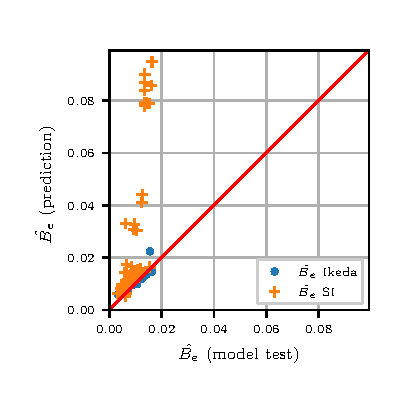
\includegraphics[width=\textwidth]{figures/si_ikeda_model.eps}
        \caption{Comparison SI, Ikeda and model tests}
        \label{fig:si_ikeda_model}
    \end{subfigure}
    ~ %add desired spacing between images, e. g. ~, \quad, \qquad, \hfill etc. 
      %(or a blank line to force the subfigure onto a new line)
    \begin{subfigure}[b]{0.4\textwidth}
        \centering
        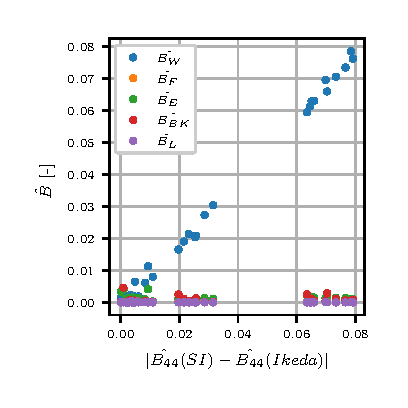
\includegraphics[width=\textwidth]{figures/component_residual.eps}
        \caption{Residual vs. components}
        \label{fig:component_residual}
    \end{subfigure}
    \newline
    ~ %add desired spacing between images, e. g. ~, \quad, \qquad, \hfill etc. 
    %(or a blank line to force the subfigure onto a new line)
    \begin{subfigure}[b]{0.4\textwidth}
        \centering
        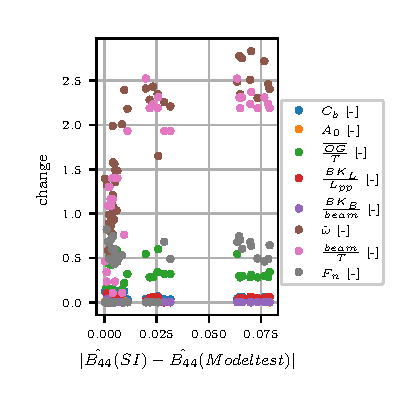
\includegraphics[width=\textwidth]{figures/parameter_residual.eps}
        \caption{Residual vs. parameters}
        \label{fig:parameter_residual}
    \end{subfigure}
    ~ %add desired spacing between images, e. g. ~, \quad, \qquad, \hfill etc. 
    %(or a blank line to force the subfigure onto a new line)
    \begin{subfigure}[b]{0.4\textwidth}
        \centering
        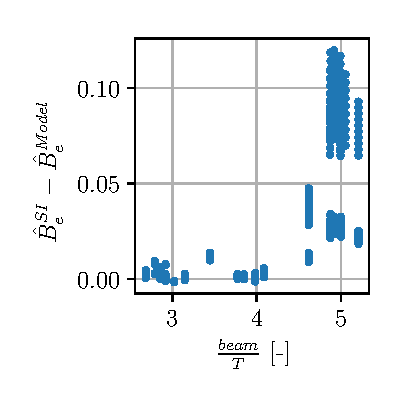
\includegraphics[width=\textwidth]{figures/beam_T_residual.eps}
        \caption{Beam to draught vs. residual}
        \label{fig:beam_T_residual}
    \end{subfigure}
    
    \caption{Analysis of the residual error of SI}\label{fig:validation}
\end{figure}



